\chapter{Aplikacja, testowanie i~dokumentacja}

Opisany w~poprzednich rozdziałach komponent Silnika odpowiedzialny jest za wyświetlanie i~sterowanie widokiem wizualizacji. Zawiera on również ich przykłady, które demonstrują różne możliwości opisu i~działania wizualizacji. Komponent Silnika budowany jest do postaci łatwej do zaimportowania biblioteki eksportującej komponent frameworka Vue.js, niezbędne interfejsy oraz przykładowe wizualizacje. Żeby w~pełni wykorzystać możliwości konfiguracji Silnika, istnieje konieczność osadzenia go w~większej aplikacji.

Rozdział ten opisuje aplikację webową typu SPA (ang. Single Page Application), która zagnieżdża komponent Silnika. Opisane zostaną również testy wizualnej regresji aplikacji oraz testy Silnika. Na końcu opisany zostanie dokumentacja Silnika.

\section{Aplikacja}
Stworzona na potrzeby projektu aplikacja webowa jest stroną typu SPA. W~większości przypadków takich aplikacji cały wykonywany kod strony pobiera się tylko raz, a~jej wygląd jest całkowicie kontrolowany przez JavaScript, który generuje odpowiednią strukturę DOMu. Podstawowa struktura projektu aplikacji została stworzona przy użyciu narzędzia \texttt{vue-cli}, co miało również miejsce dla komponentu Silnika. Tak jak to ma miejsce w~przypadku standardowych stron internetowych, tutaj również wyświetlany widok uzależniony jest od adresu URL. Zachowanie to musi być obsłużone przez JAvaScript wykorzystując History~API ~\cite{HistoryAPI} udostępniane przez przeglądarkę. Za jego integrację z~Vue.js odpowiada biblioteka \texttt{vue-router}. Strona posiada dwa widoki, które definiują dwa typy adresów.

\begin{enumerate}
    \item \texttt{/} - widok zbioru wizualizacji, pokazany na rysunku~\ref{fig:c5_visPicker}, implementowany przez komponent \texttt{VisPicker},
    \item \texttt{/visName} - widok komponentu \texttt{VisViewer}, pokazanego na rysunku~\ref{fig:c5_visViewer}, który zagnieżdża komponent \texttt{GeoVisCoreVue} wyświetlający wizualizację. \texttt{visName} to nazwa wizualizacji dostarczona do konstruktora jej klasy bazowej.
\end{enumerate}

\begin{figure}[h]
    \centering
    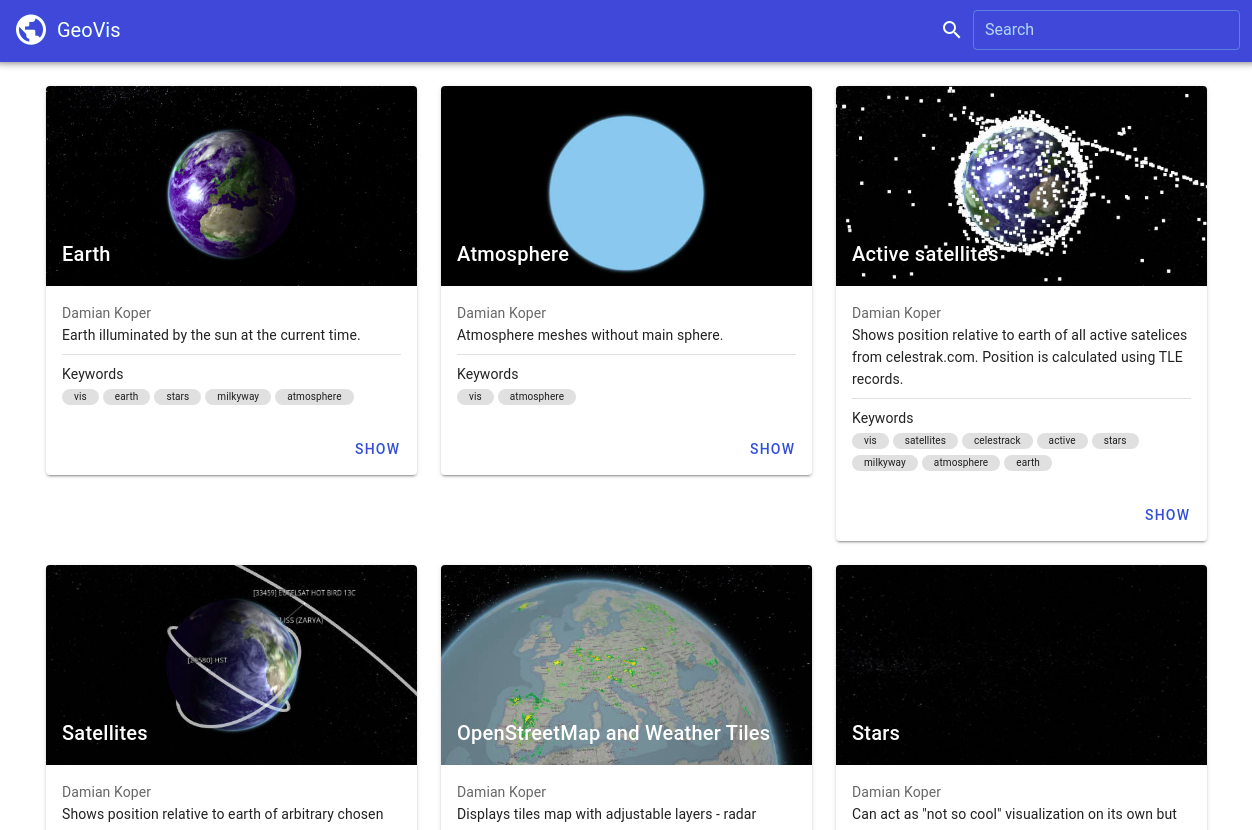
\includegraphics[width=\linewidth]{img/c5_visPicker.png}
    \caption{Widok komponentu \texttt{VisPicker} aplikacji}
    \label{fig:c5_visPicker} 
\end{figure}


Komponent \texttt{VisPicker} (rysunek~\ref{fig:c5_visPicker}) wyświetla dostarczone przez komponent Silnika wizualizacje w~postaci kart zawierających metadane - miniaturkę, tytuł, autora, opis i~słowa kluczowe. Widok ten pozwala również na filtrowanie wizualizacji. W~lewym górnym rogu interfejsu użytkownika znajduje się pole tekstowe. Po jego uzupełnieniu na ekranie pozostaną karty z~wizualizacjami, których treść dowolnej metadanej pokrywa się z~wyszukiwaną frazą. Wyświetlane karty są w~pełni responsywne. Za responsywność oraz za wygląd i~funkcjonowanie podstawowych komponentów interfejsu użytkownika odpowiada biblioteka Vuetify~\cite{Vuetify}.

\begin{figure}[h]
\centering
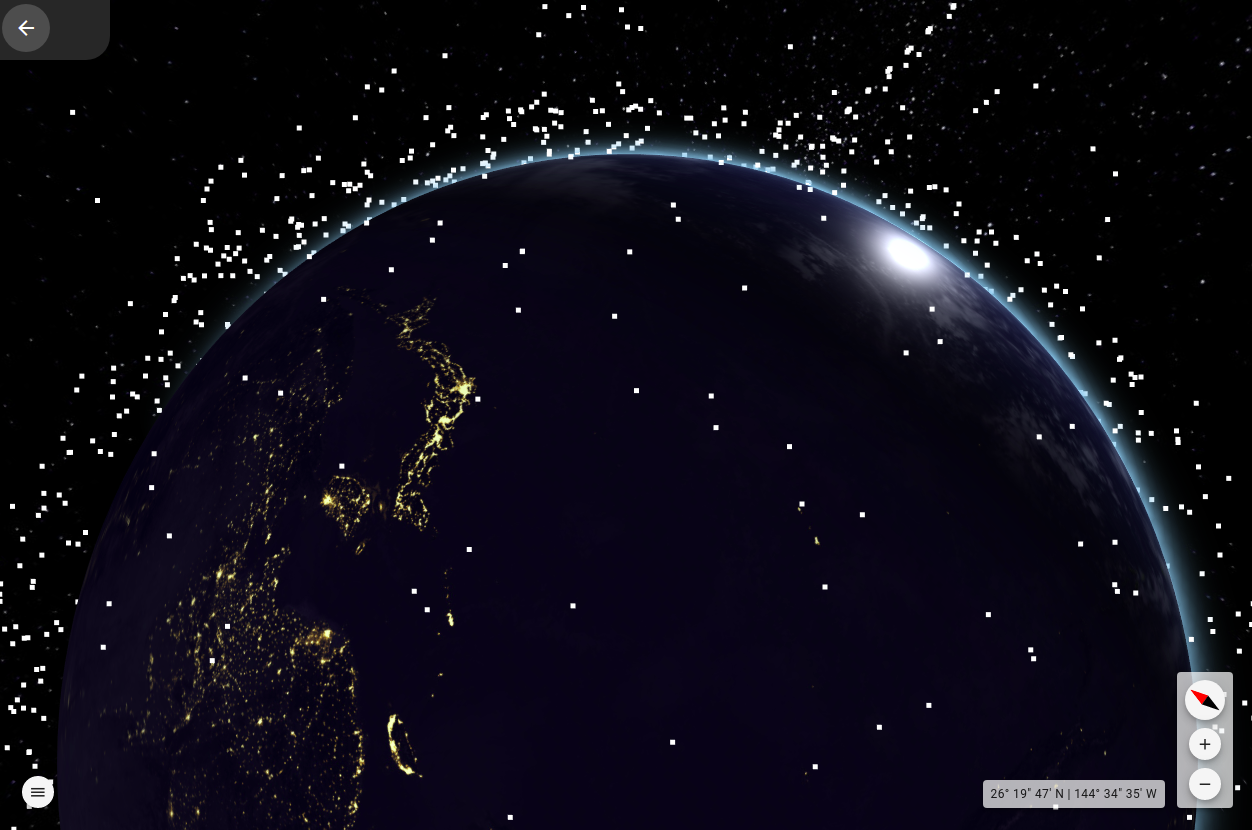
\includegraphics[width=\linewidth]{img/c5_visViewer.png}
    \caption{Widok komponentu \texttt{VisViewer} aplikacji}
    \label{fig:c5_visViewer} 
\end{figure}

Komponent \texttt{VisViewer} (rysunek~\ref{fig:c5_visViewer}) wyświetla wizualizację wybraną w~komponencie \texttt{VisPicker}. W~lewym górnym rogu widoku wyświetlany jest przycisk cofający do widoku wyboru wizualizacji.

\section{Testowanie}

Podrozdział ten opisuje proces testowania zarówno aplikacji, jak i~komponentu Silnika. Dla aplikacji stworzone zostały automatyczne testy wizualnej regresji, które charakteryzuję się tym, że w~procesie testowania bierze udział faktyczne środowisko przeglądarki. Biblioteką odpowiedzialną za te testy jest Cypress~\cite{Cypress}. Daje on możliwość kontroli zachowania przeglądarki poprzez udostępniany interfejs oraz pozwala tworzyć asercje na stan faktyczny wyświetlanego widoku poprzez analizę modelu DOM. Testy te, w~przypadku aplikacji, sprawdzają poprawność wyświetlanych metadanych w~karcie wizualizacji. Sprawdzają też mechanizm ich filtrowania.

Dla komponentu Silnika również podjęta została próba stworzenia testów wizualnej regresji. Efekt nie był jednak zadowalający. Bez problemu stworzone zostały testy sprawdzające wygląd i~funkcjonowanie elementów informacyjnych i~kontrolnych wizualizacji. Jednak do przetestowania poprawności generowanej grafiki niezbędne tutaj użycie było mechanizmu snapshotów, który w~tym wypadku porównuje piksele wygenerowanej grafiki do początkowo ustalonego wzorca. Kontrolowana przeglądarka Electron, która jest domyślną dla biblioteki Cypress, miała problemy z~wydajnością podczas ładowania bardziej złożonych wizualizacji. Zautomatyzowane testowanie wizualizacji pod kątem generowanej grafiki wymaga w~tym wypadku optymalizacji i~mechanizmów testowania, jak i~samych wizualizacji pod tym kątem.

Niektóre klasy pomocnicze w~odpowiadającym ich domenach, na których zachowaniu bazuje wiele mechanizmów posiada testy jednostkowe. Biblioteką używaną do ich wykonywania jest Jest~\cite{Jest}. Jest to najpopularniejsza biblioteka tego typu posiadająca dobrą integrację z~TypeScriptem, pozostałymi frameworkami oraz posiada łatwe w interpretacji API.

\section{Dokumentacja}

Wliczającym się w~zakres definicji narzędzie dokumentacji, ale w~procesie prac nad Silnikiem służącym do podglądu komponentu, jest narzędzie Storybook~\cite{Storybook}. Pozwala ono na szybkie prototypowanie komponentów aplikacji, tworzenie dynamicznej dokumentacji, prezentującej na żywo wygląd i~zachowanie komponentu dla podanych danych wejściowych, które użytkownik może dowolnie zmieniać. W~procesie prac nad projektem służyło ono do wyświetlania i~szybkiego przełączanie się pomiędzy przykładowymi wizualizacjami.

Narzędziem dokumentującym stworzone klasy i~zaimplementowane interfejsy komponentu Silnika jest Typedoc~\cite{Typedoc}. Wykorzystuje on informacje, które daje język TypeScript i~generuje zestaw statycznych stron, gdzie każdy moduł, każda klasa, czy też każdy interfejs bądź typ wyliczeniowy ma swoją stronę z~opisem. Dodatkowe informacje można dostarczyć zapatrując wybrany obiekt w~komentarz ze specjalnymi adnotacjami. Dokumentacja znajduje się w~katalogu \texttt{engine/docs} i~może być serwowana przez serwer plików statycznych.